%% *************************************************************************
%%
%% This is an RIT Space Exploration Standard defining guidelines for content
%% and formatting of project proposals.
%%
%% The document template SPEXformat.cls is based on the official IEEE LaTeX
%% class for authors of the Institute of Electrical and Electronics Engineers
%% (IEEE) Transactions journals and conferences.
%%
%% *************************************************************************

%% *************************************************************************
% LaTeX REFERENCES
% ----------------
%   Intro to LaTeX: http://www.rpi.edu/dept/arc/docs/latex/latex-intro.pdf
%   Comprehensive LaTeX symbol list: http://tug.ctan.org/info/symbols/comprehensive/symbols-a4.pdf
%% *************************************************************************

% tell \LaTeX what kind of formatting to use
\documentclass[journal]{SPEXformat}
% enable placeholder text generator
\usepackage{blindtext}
% enable toolbox for embedding figures and pictures
\usepackage{graphicx}
% enable package for adding a list of variables and constants at the beginning, aka "nomenclature"
\usepackage{nomencl}
% enable package for easily formatting units
\usepackage{siunitx}
% enable package for cross-referencing figures, sections, references etc.
% how to use hyperref: http://www2.washjeff.edu/users/rhigginbottom/latex/resources/lecture09.pdf
\usepackage{hyperref}
% change text encoding to make it more crisp
\usepackage[T1]{fontenc}
% enable conditionals for help text
\usepackage{etoolbox}

% ----------------------------
\newbool{showhelp}
% ~~~~~~~~~~~~~~~~~~~~~~~~~~
% SHOW HELP TEXT IN THE PDF?
\setbool{showhelp}{false}
% ~~~~~~~~~~~~~~~~~~~~~~~~~~
% define conditional help text environment
\newsavebox{\helpbox}
\newenvironment{help}{
  \ttfamily\footnotesize\sloppy
  \begin{lrbox}{\helpbox}\begin{minipage}{\linewidth}
  }{
  \end{minipage}\end{lrbox}
  \ifbool{showhelp}{
    \fbox{\usebox{\helpbox}}
  }{}
}
% ----------------------------

% initialize nomenclature package
\makenomenclature{}

% set title. choose something as descriptive and precise as possible. Descriptive > sounding cool. remember this!
\title{RIT Space Exploration Project Proposal Standard Format and Sample Content}
\author{
  \begin{help}
    List the authors of the proposal. The Champion should go first.
    The \$~\$ markers tell \LaTeX{} to treat the text inside to be treated as a math expression. This way you can use operators like \textcaret{} to place characters as superscripts.
    The \textbackslash{}thanks command puts the contents inside those brackets in a footnote at the bottom of the first page. Technically speaking, \textbackslash{}thanks is just a specially formatted footnote.
    Read here for a more advanced options:  \url{http://tex.stackexchange.com/questions/826/symbols-instead-of-numbers-as-footnote-markers}
  \end{help}
  Philip~Linden$^{*\dagger}$%
    \thanks{$^{*}$Project Champion}%
    \thanks{$^{\dagger}$BS/MEng '17, Mechanical Engineering},
  Austin~Bodzas$^{\ddagger}$%
    \thanks{$^{\ddagger}$BS '19, Computer Science},
  Drew~Walters$^{\S}$%
    \thanks{$^{\S}$BS '18, Mechanical Engineering Technology}
  % the recommended order for symbolic footnotes is
  %   (1) asterisk        *   *
  %   (2) dagger          †   \dagger
  %   (3) double dagger   ‡   \ddagger
  %   (4) section symbol  §   \S
  %   (5) paragraph       ¶   \P
  %   et cetera. For higher counts, use 2x symbols (1)-(5) (i.e. (6) two asterisks **). Keep cycling through (1)-(5) using 3x, 4x, and so on.
  %   Note that these symbol codes work in math mode and text mode.
  %   There are ways to make LaTeX do this for you, but it is more advanced and not entirely necessary, especially for short author lists. Not worth the hassle, in my opinion.
}
% page header for pages other than cover page
\markboth{Project Proposal Standard}%
{Linden \MakeLowercase{\textit{et al.}}: RIT Space Exploration}

% Initial setup is over, start building the document itself
\begin{document}
\maketitle%
% correct bad hyphenation here, separated by spaces
\hyphenation{explor-ation}

\begin{abstract}
  A standard format for SPEX Project Proposals is key to organize and document the many projects members of RIT Space Exploration wish to pursue.
  The goal of the SPEX Standard is to organize, refine, and archive space exploration research.
  Documentation is vital to sharing and maintaining the wealth of ideas and information developed by all students at RIT.\@
  SPEX Project Proposals aim to provide a foundation for new projects to grow, or premature projects to develop months or years in the future.
  A standard for project proposals and reports shall provide SPEX with a robust method to maintain a healthy ecosystem of projects in all stages of development including the event where a SPEX member goes on co-op or graduates.
    \begin{help}
      The abstract is a brief summary of the proposal. Typically it includes the purpose of the proposal, key goals or objectives, and justifications.
      Be sure not to confuse the abstract with the introduction.
      It is easiest to write the abstract after the rest of the paper has been written.
      That way you can choose key information from the sections that you've already completed and string them together in the abstract.
      Consider the abstract to be your elevator pitch to anyone reading this proposal.
      What are they reading?
      What is the goal?
      Why is it worth my time?
      The abstract is what will show up in Google results and other search engines, and what people will read when they are deciding what is worth their time and brain power.
    \end{help}
\end{abstract}

\label{sec:nomenclature}
\newcommand{\nomunit}[1]{%
\renewcommand{\nomentryend}{\hspace*{\fill}#1}}
\renewcommand{\nompreamble}{
  \begin{help}
    If you include mathematical expressions or express variables in the proposal, list them with their corresponding definitions here as a list.
    The two lines below make it look nice when defining units/values to constants.

    Note that math terms and non-math terms are separated and alphabetized, regardless of the order in which they are defined. (Recall terms \$like this\$ are in the math environment)
    Read more about advanced nomenclature formatting here:\\
    \url{https://www.sharelatex.com/learn/Nomenclatures}
  \end{help}
  }
\nomenclature{RIT}{Rochester Institute of Technology}
\nomenclature{SPEX}{RIT Space Exploration}
\nomenclature{SPP}{SPEX Project Proposal}
\nomenclature{$k$}{Linear spring stiffness coefficient}
\nomenclature{$c$}{Speed of light
 \nomunit{\,\SI{2.9979e8}{\meter\per\second}}}

\printnomenclature{}
\begin{help}
  The sections included here are required. Additional sections and subsections may be added as necessary.
\end{help}
\section{Introduction}
\label{sec:introduction}
\begin{help}
  The introduction is a place to give background and context before diving into the subject matter.
  Establish context for the work you are about to propose and the main ideas of the proposition itself.
\end{help}

\IEEEPARstart{E}{xamples} of proper formatting, organizational techniques and content make writing SPEX Project Proposals as easy and painless as possible.
Writing documentation such as proposals and reports is a lot of work, but it supports the continued growth of knowledge and experience in science and engineering for SPEX as a whole.
In technical research and academia, communicating one's thoughts and ideas is arguably more important than the ideas themselves.
For example, when applying to a grant from a scientific foundation, receiving funding to continue research impinges on how the motives and techniques of a research group resonate with the goals and objectives of the foundation.

In the case of SPEX, an SPP carries value in the act of documenting ideas and effectively communicating them with others within and external to RIT Space Exploration.

\section{Primary Objective}
\label{sec:primary-obj}
\begin{help}
  At the end of the day, whether the project ``succeeds'' or ``fails'' is judged against the objectives it sought to meet.
  Note that results that contradict expectations/hypotheses are not failures if the scientific \& engineering methods are followed along the way.
  Sometimes our expectations are wrong and that can be just as successful as getting data we thought we'd see.
  What matters are what questions you intend to answer.
  This is the main purpose or main goal the project hopes to achieve.
\end{help}

The SPEX Standard defines format and style guidelines for project documentation. The SPEX Project Proposal Standard controls these guidelines as applicable to young, exploratory ideas.

The ultimate goal of an SPP is to capture all ideas (including ones that are beyond our capability, interesting ideas, or things we just dont have time for, in addition to the ones that we actually work on and develop) and archive them such that if a student goes on coop or graduates, these ideas would not leave with them.

\begin{figure}
  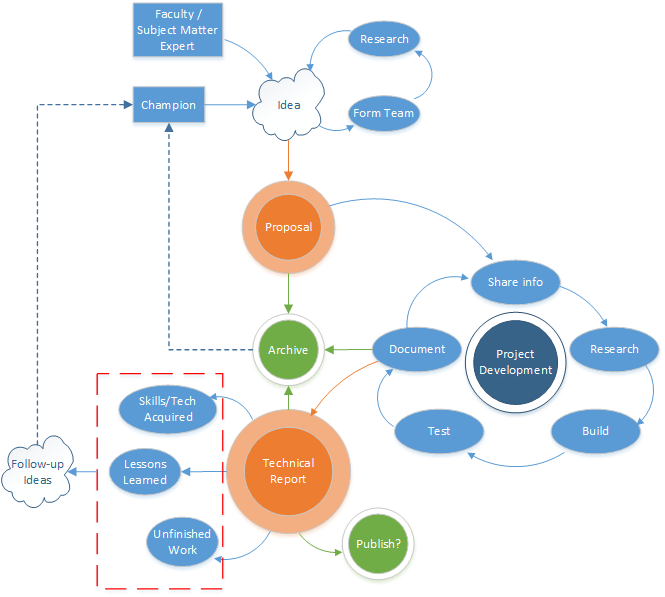
\includegraphics[width=\linewidth]{figs/project-life-cycle.png}
  \caption{An SPP is the first piece of documentation to be archived in the project life cycle. Since the life cycle can be iterative, a new proposal may also refer to one or more previous SPPs.}
\label{fig:lifecycle}
\end{figure}

% \section{Secondary Objectives}
% \label{sec:secondary-obj}

\begin{help}
  Secondary Objectives are lower priority or bonus objectives that are significant but not the main focus of the project. This template does not have secondary objectives.
\end{help}

\section{Benefit to SPEX}
\label{sec:benefit}
\begin{help}
  [this help section is not yet defined]
\end{help}

By writing proposals and familiarizing undergraduate and graduate students from any discipline with this type of approach and execution, SPEX members will be better equipped convey their ideas to others in a methodical and organized manner.
Ideally, an abundance of ideas and projects encapsulated in SPPs would outlive their respective authors and continue to sustain SPEX with valuable research opportunities invariant of individual members' absences due to co-ops or graduations.
Perhaps in the future, SPEX proposals may be used as baselines for grant applications and other funded research efforts.

\begin{help}
  Below I have used subsections to identify key ideas in this section. These particular subsections are not required as part of the SPEX Standard, but serve as an example of using subsections in a text.
\end{help}

\subsection{Mindset}
\label{subsec:mindset}
Firstly, it gets people in the right mindset for thinking about what is important and what needs to be considered before taking off on a project.
Publishing an SPP imbues a sense of formality that hopefully makes its way into the level of seriousness and merit that is desirable for SPEX to pursue.

\subsection{Traceability}
\label{subsec:traceability}
Similarly, an SPP serves to provide the foundation for traceability in requirements and objectives to projects as they grow and change.
This prevents blockers such as feature creep, rabbit holes, and spun tires, and hopefully prevents good projects from dying by getting too off track.

\subsection{Accessibility}
\label{subsec:plug-n-play}
\begin{help}
  Note below that LaTeX uses weird formatting when it comes to quotation marks.
  The style below is correct to display forward quotes \verb|``| at the start of the phrase and backquotes \verb|''| at the end.
\end{help}

Having a ``plug-and-play'' template is the first step to learning how to one's own SPP\@.
It removes a major barrier of starting from scratch, providing example content to which one could refer when creating their own.
\LaTeX{} may prove to be daunting for some people, but it is arguably better to encourage people to learn LaTeX than to rely on something like Microsoft Word.

\section{Implementation}
\label{sec:implementation}
\begin{help}
  What path do you anticipate the project to take?
\end{help}

In the ideal case, every project begins with a proposal.
That proposal gets sent around to SPEX members (and non-members) to draw support and build a team.
Research and work takes place, documented along the way until  an ending point is reached (e.g.\ project completion, end of the semester, team attrition, etc.).

At the end of the project (or end of semester, whichever comes first), the team writes a report of the project with what they did, if it was successful, and recommendations for future projects.
A future SPEX member might pick up where the last paper left off, and the cycle repeats.

\subsection{Deliverables}
\label{subsec:deliverables}
\begin{help}
  When all is said and done, what will you have to show for it?
  Examples: Hardware, software, poster, ImagineRIT demo, presentations, technical papers\ldots
\end{help}

\subsection{Milestones}
\label{subsec:milestones}
\begin{help}
  Be as detailed as you can, but it's okay if there are unknowns.
  At the very least, specify how many semester you expect the project to take until it reaches completion.
\end{help}

\section{Externalities}
\begin{help}
  Things not directly related to the work or outcomes, but related to the project as a whole.
\end{help}

\subsection{Prerequisite Skills}
\begin{help}
  Which skills do team members need to have before work can start (not including skills that will be learned ``on the job'')?
\end{help}

\subsection{Funding Requirements}
\begin{help}
  Estimate costs that would be needed to meet objectives.
\end{help}

\subsection{Faculty Support}
\begin{help}
  Identify faculty that will be involved (or would need to be involved) to meet objectives.
  Note that if a professor is the Principal Investigator (P.I.) for a project, there still needs to be a student as the SPEX Project Champion.
\end{help}

\subsection{Long-Term Vision}
\label{sec:vision}
As SPEX student members get more experience writing these papers, thr group will build a library of meaningful work and be able to save it in an organized manner.
Knowledge will be preserved and easily shared.
Perhaps SPEX Project Proposal could eventually get published, in a journal or otherwise\ldots

\section*{Acknowledgements}
The author would like to thank Dr.~Bill Destler for being an exemplary human.

\onecolumn
\appendices{}
\section{Project Life Cycle}
\begin{figure*}[h]
  \centering
  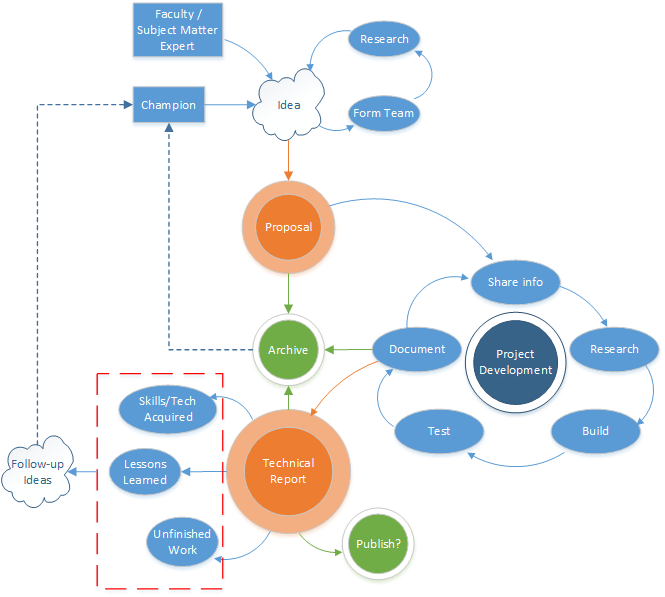
\includegraphics[]{figs/project-life-cycle.png}
  \caption{Enlarged version of the diagram in \autoref{fig:lifecycle}.}
\end{figure*}

\end{document}
